%===============================================================================
% Template Name:      SUnORE Starter Thesis/dissertation template
% Template URI:       http://sunore.co.za/sunore-thesis/
% Description:        Starter Thesis/dissertation template for SUnORE
%                     Department of Industrial Engineering,
%                     Stellenbosch University
% Version:            1.2.1
% Author:             Dr. Martin Kidd
% License:            MIT License
% License URI:        http://opensource.org/licenses/MIT
%===============================================================================
\documentclass[meng]{thesis}
% Thesis options are:
%              skripsie
%              meng
%              msc
%              mcomm
%              phdsc
%              phdcomm
%=================================================
% add packages as needed (check first, the thesis
% class already includes some packages)
%=================================================
\usepackage[figuresright]{rotating}
\usepackage{blindtext}
\usepackage{amscd,amsmath}
\usepackage{amsfonts}
\usepackage{pgfplotstable}
\usepackage{amssymb}
\usepackage{enumitem}
\usepackage{hyperref}
\usepackage{pgfplots}
\usepackage{rotating}
\usepackage{gensymb}
%=================================================
% thesis details
%=================================================
\thesistitle{Satellite Management Agent}
\student{\vspace{-8mm } by \\ \vspace{4mm} Ulrich Louw}
\graduation{September}
\gradyear{2022}
%=================================================
% if masters or skripsie
%=================================================
\supervisor{Dr HW Jordaan}
\cosupervisor{Dr JC Engelbrecht}  % remove if NA
%=================================================
% if phd
%=================================================
\promoter{Supervisor name}
\copromoter{Co-supervisor name}      % remove if NA
%=================================================
\addbibresource{bibliography.bib}     % .bib file


%=================================================
% Special Math functions
%=================================================
\newcommand{\blokkie}{\hspace{.07cm}\Box\hspace{.07cm}}


\begin{document}
	\SetKwInOut{Input}{Input}
	\SetKwInOut{Output}{Output}
	
	
	%=================================================
	% front page and decleration page - were set up
	% according to university standards (as specified
	% in yearbook) and may not be edited
	%=================================================
	\frontpage
	\dominitoc[c] % remove if you don't want mini tables of contents for each chapter
	
	
	%=================================================
	% go populate the fields in this file
	%=================================================
	
%%%%%%%%%%%%%%%%%%%%%%%%%%%%%%%%%%%%%%%%%%%%%%%%
%
% type the body of your abstracts here
%
%%%%%%%%%%%%%%%%%%%%%%%%%%%%%%%%%%%%%%%%%%%%%%%%

\engabstract{\Blindtext}

\afrabstract{Skryf jou Afrikaanse opsomming hier.}

%%%%%%%%%%%%%%%%%%%%%%%%%%%%%%%%%%%%%%%%%%%%%%%%



\ifoddmakenewpage % compensate for long abstracts



%%%%%%%%%%%%%%%%%%%%%%%%%%%%%%%%%%%%%%%%%%%%%%%%
%
% ECSA Outcome (ONLY SKRIPSIE!!)
%
%%%%%%%%%%%%%%%%%%%%%%%%%%%%%%%%%%%%%%%%%%%%%%%%
\ifthenelse{\equal{\printtype}{skripsie}}{%


\ecsa{      %ecsa outcomes
\begin{center}


\begin{tabular}{|p{8.3cm}|p{2.7cm}|p{1.5cm}|}
\hline
\headcol   & \multicolumn{2}{c|}{\textbf{Reference}} \\ \cline{2-3}
\headcol
\textbf{Outcome} & \textbf{Section} & \textbf{Page} \\ \hline
\mbox{1. Problem} solving: Demonstrate competence to identify, assess, formulate and solve convergent and divergent engineering problems creatively and innovatively. & \textit{All}  & \textit{All} \\ \hline
\rowcol
{5. Engineering methods}, skills and tools, including information technology: Demonstrate competence to use appropriate engineering methods, skills and tools, including those based on information technology. & \textit{2,3,4 \& 5}  & \textit{3--57}    \\ \hline
\mbox{6. Professional} and technical communication: Demonstrate competence to communicate effectively, both orally and in writing, with engineering audiences and the community at large.  & \textit{All}  & \textit{All}            \\ \hline
\rowcol
\mbox{9. Independent} learning ability: Demonstrate competence to engage in independent learning through well developed learning skills. & \textit{2,3,4 \& 5} & \textit{3--57}  \\ \hline
\mbox{10. Engineering} professionalism: Demonstrate critical awareness of the need to act professionally and ethically and to exercise judgement and take responsibility within own limits of competence.  & \textit{All}                 & \textit{All}  \\ \hline
\end{tabular}
\end{center}
}
\ifoddmakenewpage
}{}%



%%%%%%%%%%%%%%%%%%%%%%%%%%%%%%%%%%%%%%%%%%%%%%%%
%
% list your acknowledgements here
%
%%%%%%%%%%%%%%%%%%%%%%%%%%%%%%%%%%%%%%%%%%%%%%%%
\acknowledgements{
\begin{itemize}
\item 
\item 
\item 
\end{itemize}
}

%%%%%%%%%%%%%%%%%%%%%%%%%%%%%%%%%%%%%%%%%%%%%%%%


\ifoddmakenewpage % compensate for long acknowledgements




\tableofcontents




%%%%%%%%%%%%%%%%%%%%%%%%%%%%%%%%%%%%%%%%%%%%%%%%%%%%%%%%%%%%
%
% populate your glossary here - remove if you dont want one
%
%%%%%%%%%%%%%%%%%%%%%%%%%%%%%%%%%%%%%%%%%%%%%%%%%%%%%%%%%%%%

\Glossary % makes the heading

\begin{description}
\item[Something] Description of that something.
\item[Something] Description of that something.
\item[Something] Description of that something.
\end{description}


%%%%%%%%%%%%%%%%%%%%%%%%%%%%%%%%%%%%%%%%%%%%%%%%%%%%%%%%%%%%


\ifoddmakenewpage





%%%%%%%%%%%%%%%%%%%%%%%%%%%%%%%%%%%%%%%%%%%%%%%%%%%%%%%%%%%%%%%%%%%%
%
% populate your list of symbols here - remove if you dont want one
%
%%%%%%%%%%%%%%%%%%%%%%%%%%%%%%%%%%%%%%%%%%%%%%%%%%%%%%%%%%%%%%%%%%%%


\listofsymbols % makes the heading


\begin{fontconventions}
$A$       &   Symbol denoting a {\bf some general thing}   &   (Roman capitals)\\
$\cal A$  &   Symbol denoting a {\bf some general thing}   &   (Calligraphic capitals)\\ 
\end{fontconventions}


\begin{symboltable}
$\times$ & Symbol used to denote the multiplication operator \\
$\times$ & Symbol used to denote the multiplication operator \\
$\times$ & Symbol used to denote the multiplication operator \\
$\times$ & Symbol used to denote the multiplication operator \\
$\times$ & Symbol used to denote the multiplication operator \\ 
\end{symboltable}


%%%%%%%%%%%%%%%%%%%%%%%%%%%%%%%%%%%%%%%%%%%%%%%%%%%%%%%%%%%%%%%%%%%%


\ifoddmakenewpage




%%%%%%%%%%%%%%%%%%%%%%%%%%%%%%%%%%%%%%%%%%%%%%%%%%%%%%%%%%%%%%%%%%%%
%
% populate your list of acronyms here - remove if you dont want one
%
%%%%%%%%%%%%%%%%%%%%%%%%%%%%%%%%%%%%%%%%%%%%%%%%%%%%%%%%%%%%%%%%%%%%


\listofacronyms % makes the heading


\begin{description}
\item[ADCS:] Attitude Determination and Control System
\item[SGP4:] Simplified General Perturbations 4
\item[UAV:] Unmanned Aerial Vehicle
\item[EFC:] Earth Fixed Coordinate
\item[EIC:] Earth Inertial Coordinate
\item[ORC:] Orbit-referenced Coordinate 
\item[SBC:] Satellite Body Coordinate
\item[SPCC:] Squared Pearson Correlation Coefficient
\item[BST:] Binary Search Tree
\item[IGRF:] International Geomagnetic Reference Field
\item[FDIR:] Fault Detection, Isolation and Recovery
\item[FDIR:] What It Stands For
\item[FDIR:] What It Stands For
\item[FDIR:] What It Stands For
\item[FDIR:] What It Stands For
\item[FDIR:] What It Stands For
\item[FDIR:] What It Stands For

\end{description}


%%%%%%%%%%%%%%%%%%%%%%%%%%%%%%%%%%%%%%%%%%%%%%%%%%%%%%%%%%%%%%%%%%%%



\ifoddmakenewpage




%%%%%%%%%%%%%%%%%%%%%%%%%%%%%%%%%%%%%%%%%%%%%%%%
%
% lists - remove what you dont need
%
%%%%%%%%%%%%%%%%%%%%%%%%%%%%%%%%%%%%%%%%%%%%%%%%

\listoffigures
\ifoddmakenewpage
\listoftables
\ifoddmakenewpage
\listofalgorithms
\ifoddmakenewpage
%%%%%%%%%%%%%%%%%%%%%%%%%%%%%%%%%%%%%%%%%%%%%%%%
	
	
	%=================================================
	% how-to examples:
	%=================================================
	%%%%%%%%%%%%%%%%%%%%%%%%%%%%%%%%%%%%%%%%%%%%%%%%%
%
% some tips on creating nice tables
%
%%%%%%%%%%%%%%%%%%%%%%%%%%%%%%%%%%%%%%%%%%%%%%%%
\chapter{Tables}


% TABLE SHADING
%===============
%
% uncomment to change the default shades (gray!45 and gray!25) for the tables in your thesis:
%    \colorlet{tableheadcolor}{gray!45}  % headers
%    \colorlet{tablerowcolor}{gray!25}   % normal rows
%
% \headcol                 - for shading the header of your table
% \rowcol                  - shades an entire row
% \rowcolor{color}         - for custum coloring of a row
%
% \cellcolrow              - shades a single entry in the table the shade of a row
% \cellcolhead             - shades a single entry in the table the shade of the header
% \cellcolor{color}        - for custom colouring of a single entry in the table
%
% \rowcolors{startrow}{oddrowcolor}{evenrowcolor} - for automatic shading of rows, put in table environment
%   examples:
%     \rowcolors{3}{gray!25}{} - shades 3rd row and every second row after that
%     \rowcolors{2}{}{gray!25} - shades 2rd row and every second row after that




% TABLE LINES
%=============
%
% \toprule     - the top-most line of a table, does not work with shading
% \hline       - normal line, does not work with shading
% \midline     - normal line, does not work with shading
% \bottomrule  - a line for the bottom of the table, does not work with shading
%
% \topline     - the top-most line of a table if the header is shaded
%
% \midline     - the line between the headings and the table body
% \midlinecbw  - a line for when the previous row is rowcolor and the next line is white
% \midlinecw   - a line with no black, to further separate a rowcolor row and a white row
% \midlinewbc  - a line for when the upper row is white and the next line is rowcolor
% \midlinewc   - a line with no black, to further separate a white row and a rowcolor row
%
% \bottomline  - a line for the bottom of the table, when the last row is white
% \bottomlinec - a line for the bottom of the table, when the last row is rowcolor

% EXAMPLE
%========

\begin{table}[htb!]
	\centering
		\begin{tabular}{rrrr|rrrrrr}
   \topline    \headcol\multicolumn{4}{c|}{Results for ${\cal P}_{n} \blokkie {\cal P}_n$}&\multicolumn{4}{c}{Results for ${\cal H}_{n,n}$}\\
    \headcol $n$	&	LP	&	$\gamma_s$	&	Time		&	$n$	&	LP	&	$\gamma_s$	&	Time	\\	\midline
2	&	1.33	&	2	&	0.01	&		2	&	1.00	&	2	&	0.01	\\	\rowcol
3	&	2.50	&	4	&	0.02	&		3	&	2.00	&	3	&	0.01	\\	
4	&	4.00	&	7	&	0.07	&		4	&	4.00	&	5	&	0.04	\\	\rowcol
5	&	6.27	&	9	&	0.17	&		5	&	5.00	&	7	&	0.08	\\	
6	&	8.75	&	13	&	0.39	&		6	&	6.00	&	10	&	0.27	\\	\rowcol
7	&	11.50	&	18	&	2.90	&		7	&	9.00	&	13	&	7.41	\\	
8	&	14.81	&	23	&	72.16	&		8	&	11.33	&	17	&	110.00	\\	\rowcol
9	&	18.25	&	29	&	23\,356.24		&	9	&	13.50	&	21	&	1\,083.17	\\	
10	&	22.39	&	35$^*$	&	TO	&		10	&	16.86	&	27$^\dagger$	&	MO	\\	\bottomline

		\end{tabular}
%\vspace{0.5cm}
	\caption[Do not end short caption with full-stop]{Each table must be supplied with a long caption, making the table stand-alone (e.g.\ \mbox{describing} the meaning of all symbols, rows and columns), ended with a full-stop.}
	\label{tab:StaticResults}
\end{table}




% EXAMPLE
%=========
%
% example using multicolumn, multirow and the sideways environment

\begin{table}[h!tb]

\centering

\begin{tabular}{cc|rrrrrr}\hline

\headcol &&\multicolumn{6}{c}{this goes across 6 columns}\\

 \headcol && col a & col b & col c & col d & col e & col f \\ \hline \hline

\multirow{6}{*}{
%
\begin{sideways}
this is sideways,
\end{sideways}
%
\begin{sideways}
and goes across
\end{sideways}
%
\begin{sideways}
six rows
\end{sideways}
%
}


& row 1 \\
& row 2 & \cellcolrow & \cellcolrow & \cellcolrow & \cellcolrow & \cellcolrow & \cellcolrow \\
& row 3 \\ 
& row 4 & \cellcolrow & \cellcolrow & \cellcolrow & \cellcolrow & \cellcolrow & \cellcolrow \\
& row 5 \\
& row 6 & \cellcolrow & \cellcolrow & \cellcolrow & \cellcolrow & \cellcolrow & \cellcolrow \\ \hline

\end{tabular}

\caption[Do not end short caption with full-stop]{Type full caption here.}
\label{ex2}

\end{table}


 \begin{table}[htb]
\begin{center}
\begin{tabular}{crrrrrrrrr}
    \topline\headcol
$n\ \rightarrow$	&	$2$	&	$3$	&	$4$	&	$5$	&	$6$	&	$7$	&	$8$&$9$	\\\midline
$|{\cal S}_n^0|$	&	1	&	2	&	6	&	17	&	81	&	514	&	5\,460	&107\,794\\\rowcol
$|{\cal S}_n^1|$	&		&	1 	&	3 &	10 &	51 	&	355 	&	4\,205&94\,106 	\\
$|{\cal S}_n^2|$	&		&		&	1 	&	4 	&	16 	&	136 	&	2\,050&52\,502 	\\\rowcol
$|{\cal S}_n^3|$	&		&		&		&	2 	&	5	&	32 	&	551 &16\,923	\\
$|{\cal S}_n^4|$	&		&		&		&		&	2 	&	5 	&	70  &3\,081	\\\rowcol
$|{\cal S}_n^5|$	&		&		&		&		&		&	1 	&	6 &245	\\
$|{\cal S}_n^6|$	&		&		&		&		&		&		&	3 &13\\\rowcol
$|{\cal S}_n^7|$	&		&		&		&		&		&		&	 &3
\\\midlinecbh\headcol Total &1&3&10&33&155&1\,043&12\,345&274\,667\\
\headcol Time&&$\ll1$&$<1$&1&15&374&15\,895&1\,069\,220\\\bottomlinect
\end{tabular}
\end{center}
\vspace{-0.5cm}
\caption[Do not end short caption with full-stop]{Type full caption here.}
\label{Tab:StabResults}
\end{table}





             % remove if NA
	%%%%%%%%%%%%%%%%%%%%%%%%%%%%%%%%%%%%%%%%%%%%%%%%%
%
% figures - https://www.sharelatex.com/learn/Inserting_Images
%
%%%%%%%%%%%%%%%%%%%%%%%%%%%%%%%%%%%%%%%%%%%%%%%%
\chapter{Figures}


% BASIC EXAMPLE
%================

\begin{figure}[h!tb]
\centering

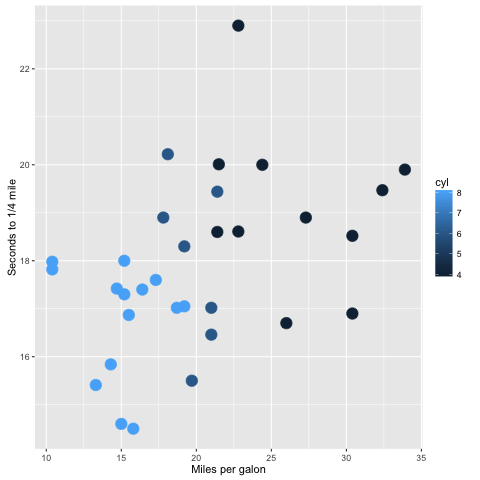
\includegraphics[width=10cm]{fig/plot1} % not necessary to give extension - now you can shift between compiling to ps or to pdf without any problems
 
\caption[Do not end short caption with full-stop]{Each figure must be supplied with a long caption, making the figure stand-alone and ended with a full-stop.}

\end{figure}





\newpage





% SUBFIG EXAMPLE
%================
%
% usage: \subfloat[][caption]{...figure code...\label{label}}

The subfigures are Figures \subref{firstfigure}, \subref{secondfigure}, \subref{thirdfigure} and \subref{fourthfigure}.

\begin{figure}
\centering

\subfloat[][First subcaption (No full-stop)]{
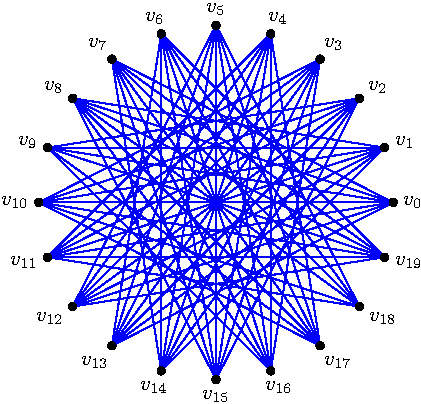
\includegraphics{fig/figure}
\label{firstfigure}
}
\quad
\subfloat[][Second subcaption (No full-stop)]{
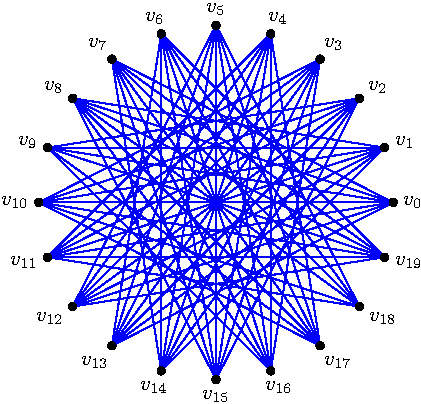
\includegraphics{fig/figure}
\label{secondfigure}
}
\\
\subfloat[][Third subcaption (No full-stop)]{
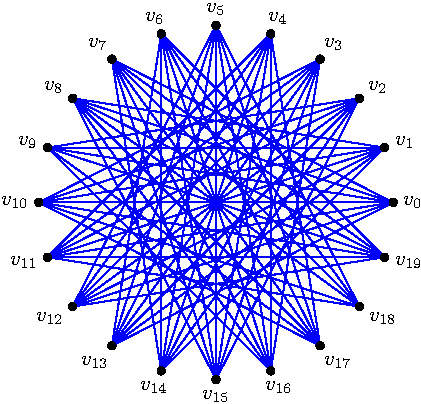
\includegraphics{fig/figure}
\label{thirdfigure}
}
\quad
\subfloat[][Fourth subcaption (No full-stop)]{
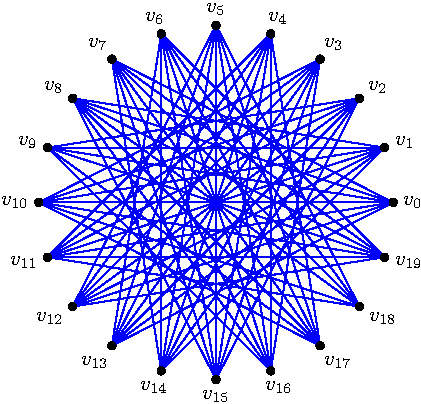
\includegraphics{fig/figure}
\label{fourthfigure}
}
\caption[Do not end short caption with full-stop]{End the main caption with a full-stop, but not each of the sub-figure captions!}
\label{thislabel}
\end{figure}
            % remove if NA
	%%%%%%%%%%%%%%%%%%%%%%%%%%%%%%%%%%%%%%%%%%%%%%%%%
%
% how to typeset algorithms
%
%%%%%%%%%%%%%%%%%%%%%%%%%%%%%%%%%%%%%%%%%%%%%%%%
\chapter{Algorithms}

% USE THE TEMPLATE BELOW FOR YOUR ALGORITHMS
%============================================
%
% \begin{algorithm}
% 
% \SetKwInOut{Input}{Input}
% \SetKwInOut{Output}{Output}
% 
% \Indm
% \Input{Description of the input to the algorithm.}
% \Output{Description of the output from the algorithm.}
% \Indp
% 
% \BlankLine
% 
%   % main algorithm code here
% 
% \caption{Algorithm example}
% \label{alg}
%
% \end{algorithm}



\begin{algorithm}

\SetKwInOut{Input}{Input}
\SetKwInOut{Output}{Output}

\SetKwData{Left}{left}
\SetKwData{This}{this}
\SetKwData{Up}{up}
\SetKwFunction{Union}{Union}
\SetKwFunction{FindCompress}{FindCompress}

\Indm
\Input{Description of the input to the algorithm.}
\Output{Description of the output from the algorithm.}
\Indp

\BlankLine

\emph{special treatment of the first line}\;
\For{$i\leftarrow 2$ \KwTo $l$}{
  \emph{special treatment of the first element of line $i$}\;
  \For{$j\leftarrow 2$ \KwTo $w$}{\label{forins}
    \Left$\leftarrow$ \FindCompress{$Im[i,j-1]$}\;
    \Up$\leftarrow$ \FindCompress{$Im[i-1,]$}\;
    \This$\leftarrow$ \FindCompress{$Im[i,j]$}\;
    \If{\Left compatible with \This}{\label{lt}
      \lIf{\Left $<$ \This}{\Union{\Left,\This}}\;
      \lElse{\Union{\This,\Left}\;}
    }
    \If{\Up compatible with \This}{\label{ut}
      \lIf{\Up $<$ \This}{\Union{\Up,\This}}\;
      \lElse{\Union{\This,\Up}}
    }
  }
  \lForEach{element $e$ of the line $i$}{\FindCompress{p}}
}

\caption[Do not end short caption with full-stop]{Algorithm example}
\label{alg}

\end{algorithm}




\begin{algorithm}[t]
%\SetAlgoNoLine
 \Input{A tree $T$ represented by an array {\sf Parent}$[1,\ldots,n]$.}
\Output{A minimum secure dominating set of $T$, represented by a boolean array $X$.}
\For{$i\leftarrow 1$ to $n$}{
{\sf A3Label}$[i] \leftarrow$ {\sc False}\;
$X[i] \leftarrow$ {\sc F\SetKwInOut{Input}{Input}
	\SetKwInOut{Output}{Output}
	
	\SetKwData{Left}{left}
	\SetKwData{This}{this}
	\SetKwData{Up}{up}
	\SetKwFunction{Union}{Union}
	\SetKwFunction{FindCompress}{FindCompress}
	
	\Indm
	\Input{Description of the input to the algorithm.}
	\Output{Description of the output from the algorithm.}
	\Indp
	
	\BlankLine
	
	\emph{special treatment of the first line}\;
	\For{$i\leftarrow 2$ \KwTo $l$}{
		\emph{special treatment of the first element of line $i$}\;
		\For{$j\leftarrow 2$ \KwTo $w$}{\label{forins}
			\Left$\leftarrow$ \FindCompress{$Im[i,j-1]$}\;
			\Up$\leftarrow$ \FindCompress{$Im[i-1,]$}\;
			\This$\leftarrow$ \FindCompress{$Im[i,j]$}\;
			\If{\Left compatible with \This}{\label{lt}
				\lIf{\Left $<$ \This}{\Union{\Left,\This}}\;
				\lElse{\Union{\This,\Left}\;}
			}
			\If{\Up compatible with \This}{\label{ut}
				\lIf{\Up $<$ \This}{\Union{\Up,\This}}\;
				\lElse{\Union{\This,\Up}}
			}
		}
		\lForEach{element $e$ of the line $i$}{\FindCompress{p}}
	}
	
	\caption[Do not end short caption with full-stop]{Algorithm example}
	\label{alg}
	alse}\;
{\sf Labels}$[i] \leftarrow [0,0,0,0,0,0,0]$\;
{\bf if} vertex $i$ is a anchor of $T$ {\bf then} {\sf Branch}$[i] \leftarrow$ {\sc True}\;
{\sf Previous1Label}$[i] \leftarrow 0$\;
}
\For{$i\leftarrow n$ down to $2$}{
$\ell \leftarrow$ {\sf\bf EffectiveLabel}({\sf Labels}[$i$])\;
{\bf if} $\ell$ is odd {\bf then} $X[i] \leftarrow ${\sc True}\;
{\sf Labels$[$Parent$[i],\ell(i)+1 \ (\rm{mod}\ 7)]$} $++$\;
\If{$\ell=2$ {\bf and} {\sf Branch$[$Parent$[i]]$}}{
{\sf A3Label[Parent}$[i]] \leftarrow$ {\sc True}\;
{\sf prev} $\leftarrow$ {\sf Previous1Label$[$Parent$[i]]$}\;
{\bf if} {\sf prev} $>0$ {\bf then} $X[${\sf prev}$] \leftarrow$ {\sc True}\;
}
\If{$\ell=0$ {\bf and} {\sf Branch$[$Parent$[i]]$}}{
\If{{\sf A3Label$[$Parent$[i]]$}}{
$X[i] \leftarrow$ {\sc True}\;
}
\Else{
{\sf prev} $\leftarrow$ {\sf Previous1Label$[$Parent$[i]]$}\;
{\bf if} {\sf prev} $>0$ {\bf then} $X[${\sf prev}$] \leftarrow$ {\sc True}\;
{\sf Previous1Label$[$Parent$[i]] \leftarrow i$}\;
}
}
}
$\ell \leftarrow$ {\sf\bf EffectiveLabel}({\sf Labels}[$1$])\;
{\bf if} $\ell$ is odd {\bf then} $X[1] \leftarrow ${\sc True}\;
{\bf if}  {\sf Labels}$[1,j]=0$ for $j=1,3,4,5,6$ {\bf then} $X[1] \leftarrow$ {\sc True}\;
{\bf if} {\sf Labels}$[1,j]=0$ for $j=1,3,5,6$ {\bf and} {\sf Labels}$[1,0] \geq |${\sf Labels}$[1]-1|$  {\bf then} $X[1] \leftarrow$ {\sc True}\;
\If{$\ell=3$}{
{\sf prev} $\leftarrow$ {\sf Previous1Label$[1]$}\;
{\bf if} {\sf prev} $ > 0$ {\bf then} $X[$\sf{prev}$]$ $\leftarrow$ {\sc True}\;
}
\Return[$X$]\;
\caption[{{Do not end short caption with full-stop}}]{{\sf\bf DefendTree}}
\label{Alg:Tree}
\end{algorithm}

         % remove if NA
	
	
	%=================================================
	% include your chapters here
	%=================================================
	%%%%%%%%%%%%%%%%%%%%%%%%%%%%%%%%%%%%%%%%%%%%%%%%
%
% start writing
%
%%%%%%%%%%%%%%%%%%%%%%%%%%%%%%%%%%%%%%%%%%%%%%%%


\chapter{Introduction}
% put these two lines after every \chapter{} command
\vspace{-2em}
\minitoc

\startarabicpagenumbering % must be just after the first \chapter{} command


\blindtext

\section{Background}

\blindtext

\blindtext

\section{Informal problem description}

\blindtext

\blindtext

\section{Research hypothesis}

\Blindtext

\section{Scope and objectives}

The following objectives will be pursued in this project/thesis/dissertation:
\begin{enumerate}[label=\Roman*]										% \usepackage{enumitem}
 \item To \textit{conduct} a thorough survey of the literature related to:
 \begin{enumerate}[label=(\alph*)]
  \item facility location problems in general,
  \item models for the placement of a network of radio transmitters in particular,
  \item the nature of parameters required to describe effective radio transmission, and
  \item terrain elevation data required to generate an instance of the bi-objective radio transmitter location problem described in the previous section.
 \end{enumerate}
 \item  To \textit{establish} an suitable framework for evaluating the effectiveness of a given set of placement locations for a network of radio transmitters in respect of its total area coverage and its mutual area coverage.
 \item To \textit{formulate} a bi-objective facility location model suitable as a basis for decision support in respect of the location of a network of radio transmitters with a view to identify high-quality trade-offs between maximising total coverage area and maximising mutual coverage area.  The model should take as input the parameters and data identified in Objective~I(c)--(d) and function within the context of the framework of Objective~II.
 \item To \textit{design} a generic \textit{decision support system} (DSS) capable of suggesting high-quality trade-off locations for user-specified instances of the bi-objective radio transmitter location problem described in the previous section.  This DSS should incorporate the location model of Objective~III.
 \item To \textit{implement} a concept demonstrator of the DSS of Objective IV in an applicable software platform.  This DSS should be flexible in the sense of being able to take as input an instance of the bi-objective radio transmitter location problem described in the previous section via user-specification of the parameters and data of Objectives I(c)--(d) and produce as output a set of high-quality trade-off transmitter locations for that instance.
 \item To \textit{verify} and validate the implementation of Objective V according to generally accepted modelling guidelines.
 \item To \textit{apply} the concept demonstrator of Objective V to a special case study involving realistic radio transmission parameters and real elevation data for a specified portion of terrain.
 \item To \textit{evaluate} the effectiveness of the DSS and associated concept demonstrator of Objectives~IV--VI in terms of its capability to identify a set of high-quality trade-off solutions for a network of radio transmitter locations.
 \item To \textit{recommend} sensible follow-up work related to the work in this project which may be pursued in future.
\end{enumerate}

\section{Research methodology}
\blindtext

\section{Project/thesis/dissertation organisation}
\blindtext
	\chapter{Literature Study}
% put these two lines after every \chapter{} command
\vspace{-2em}
\minitoc

The implementation of FDIR on satellites have multiple complications with regards to the type of data generated by a satellite and the methodologies that can be implemented within the time and memory constraint of a cube-sat processor.

\section{Anomaly Detection on Satellites}
Various methodologies have been tested on different component of satellites. Therefore a summary of these research articles are provided in this section.

\subsection{Analysis and Prediction of Satellite Anomalies}
\textcite{Wintoft}

\subsection{Agent-based algorithm for fault detection and recovery of gyroscope's drift in small satellite missions}
To ensure that the ADCS of satellites are autonomous every aspect of the control must be able to recover from faults. \textcite{carvajal2017agent} developed an algorithm to evaluate the control of a gyroscope and detect whether drifting exists. If drifting is detected another algorithm is deployed to ensure the recovery of the gyroscope drift by updating the error state vector.

\subsection{Multivariate Anomaly Detection in Discrete and Continuous Telemetry Signals Using a Sparse Decomposition in a Dictionary}
\cite{Pilastre2020}

\subsection{Fault isolation of reaction wheels onboard three-axis controlled in-orbit satellite using ensemble machine learning}
\cite{rahimi2020fault}

\subsection{Fault tolerant control for satellites with four reaction wheels}
\cite{jin2008fault}

\subsection{Innovative Fault Detection, Isolation and Recovery Strategies On-Board Spacecraft: State of the Art and Research Challenges}
\cite{wander2013innovative}

\subsection{Machine learning methods for spacecraft telemetry mining}
\cite{ibrahim2018machine}

\subsection{Machine learning techniques for satellite fault diagnosis}
\cite{ibrahim2020machine}

\section{Statistical Methods}
\subsection{Pearson Correlation}
Vectors of certain sensors are highly correlated. For instance the vector of the earth sensor is highly correlated since the magnitude of the vector remains more or less constant. To detect anomalies the correlation of vectors can be measured and with a specified threshold the correlation can be indicated as a anomaly or nor.

The squared Pearson correlation coefficient (SPCC) for vectors depicted as
\linebreak
\\
\centerline{$a = [a_1, a_2, \ldots, a_L]^T,$}
\linebreak
\centerline{$b = [b_1, b_2, \ldots, b_L]^T,$}
\\
is defined as \cite{benesty2009pearson}
\begin{equation}
	\rho^2 (a,b) = \frac{E^2 (a,b)}{E(a^Ta)E(b^Tb)}.
\end{equation}
The correlation coefficient is proven to be constraint as
\begin{equation}
	0 \leq \rho \leq 1,
\end{equation}
where $\rho = 1$ is perfect linear correlation. 

\subsection{Variance}
Within a sequential data sample of the satellite, the variance of the variables should be within a given threshold if the satellite is in a stable condition. The variance of the data sample is defined as 
\begin{equation}
	S^2 = \frac{\sum(x_i + \bar{x})^2}{n-1}
\end{equation}
where $x$ defines the variable within the dataset.

\subsection{Kalman-Filter}
The Kalman-filter application would require the state-space matrices to be provided in the log file.

\subsection{Multivariate Guassian Distribution}
The assumption that the error of our data is generated with a Guassian distribution with a specific mean, $\mu$, and variance, $\sigma^2$, provides the opportunity for using multi-variate Gaussian distribution to determine the probability of a data-sample within a dataset. 
\begin{equation}
	\label{mean}
	\mu_j = \frac{1}{m} \sum_{i=1}^{m}x_j^{(i)}
\end{equation}

\begin{equation}
	\label{variance}
	\sigma_j^2 = \frac{1}{m} \sum_{i=1}^{m}(x_j^{(i)} - \mu_j)^2
\end{equation}

\begin{equation}
	\label{guassian distribution}
	p(x) = \prod_{j=1}^{n} \frac{1}{\sqrt{2\pi}\sigma_j}exp(-\frac{(x_j-\mu_j)^2}{2\sigma_j^2})
\end{equation}

For multi-variate Guassian distribution \cite{do2008multivariate}.

\begin{equation}
	\label{sum}
	\sum = \frac{1}{m}\sum_{i=1}^{m}(x^{(i)}-\mu)(x^{(i)}-\mu)^T
\end{equation}

\begin{equation}
	\label{multi-variate guassian distribution}
	p(x) = \frac{1}{(2\pi)^{\frac{n}{2}}{\lvert \sum \rvert}^\frac{1}{2}} exp(-\frac{1}{2}(x-\mu)^T{\sum}^{-1}(x-\mu))
\end{equation}

The Anomalies will be classified based on probabilities smaller than a given threshold $p(x) < \epsilon$.

\begin{algorithm}
	\SetKwInOut{Input}{Input}
	\SetKwInOut{Output}{Output}
	
	\SetKwData{Left}{left}
	\SetKwData{This}{this}
	\SetKwData{Up}{up}
	\SetKwFunction{Union}{Union}
	\SetKwFunction{FindCompress}{FindCompress}
	
	\Indm
	\Input{Data sample from satellite orbit.}
	\Output{Whether dataset contains anomaly.}
	\Indp
	\BlankLine
	
	Determine feature vectors $x_i$ \\
	Determine threshold probabilty, $\epsilon$ \\
	Calculate $\mu_j$ with Eq~\ref{mean} \\
	Calculate $\sigma_j$ with Eq~\ref{variance} \\
	Calculate $p(x)$ with Eq~\ref{guassian distribution} \\
	\If{$p(x) < \epsilon$}{Anomaly $= True$}
	\Else{Anomaly $= False$}
	
	\caption[Multi-variate Guassian Distribution]{Multi-variate Guassian Distribution Algorithm}
	\label{alg}
\end{algorithm}

\subsection{Kullback-Leibler Divergence}
The Kullback-Leibler divergence quantifies the difference between two probability density functions, denoted as $p(x)$ and $q(x)$ \cite{hershey2007approximating}. Satellites are systems that are predictable within a time-series. The divergence between two sequential data buffers from the satellite will have a very similar probability distribution. Therefore calculating the difference between two datasets can be used to detect an anomaly based on a given threshold.

The difference between the probability distributions from datasets, $a$ and $b$, in Figure~\ref{Guassian plot} cannot simply be calculated as the difference in the mean or the difference in the variance. To overcome this, the divergence between the two distributions can be calculated. Intuitively a point $x$ with a high probability in the dataset $a$ should have a high probability in the dataset $b$ if the two datasets have a small divergence. 

\pgfmathdeclarefunction{gauss}{3}{%
	\pgfmathparse{1/(#3*sqrt(2*pi))*exp(-((#1-#2)^2)/(2*#3^2))}%
}
\begin{figure}[!h]
	\centering
	\textbf{Difference Between Probability Distributions}
	\begin{tikzpicture}
		\begin{axis}[
			no markers, 
			domain=-3:6, 
			samples=100,
			ymin=0,
			axis lines*=left, 
			xlabel=$x$,
			every axis y label/.style={at=(current axis.above origin),anchor=south},
			every axis x label/.style={at=(current axis.right of origin),anchor=west},
			height=5cm, 
			width=12cm,
			xtick=\empty, 
			ytick=\empty,
			enlargelimits=false, 
			clip=false, 
			axis on top,
			grid = major,
			hide y axis
			]
			
			\addplot [very thick,cyan!50!black] {gauss(x, 3, 1)};
			
			\pgfmathsetmacro\valueA{gauss(3,3,1)}
			\draw [gray] (axis cs:3,0) -- (axis cs:3,\valueA);
			
			\node[below] at (axis cs:3, 0)  {$\mu_p$}; 
			
			\addplot [very thick,red!50!black] {gauss(x, 1.5, 1.5)};
			
			\pgfmathsetmacro\valueB{gauss(1.5,1.5,1.5)}
			\draw [gray] (axis cs:1.5,0) -- (axis cs:1.5,\valueB);
			
			\node[below] at (axis cs:1.5, 0)  {$\mu_q$}; 
		\end{axis}
		
	\end{tikzpicture}
	\caption{Guassian Distributions}
	\label{Guassian plot}
\end{figure}

The divergence can be expressed as 

\begin{equation}
	KL(P\lvert\lvert Q) = \int p(x) \log \left( \frac{q(x)}{p(x)} \right)dx.
\end{equation}

\subsection{Canonical Correlation Analysis}
Due to the orbital nature of satellites there exist a correlation between various sensors. For instance the sun sensor, magnetometer and earth sensor are correlated based on the desired orientation and orbit of the satellite. This correlation might not be of linear nature, but with non-linear correlation methods such as kernel canonical correlation the correlation can be measured.

However, canonical correlation provides the measure of correlation between a multi-dimensional variable with another multi-dimensional variable. Although this seems profitable for satellite fault detection, it will only be applicable for each the comparison between individual sensors. This will indicate the non-linear correlation of the sun sensor with regards to the magnetometer. The problem however, according to \textcite{chen2017fault} is to, determine the appropriate threshold for which to classify a fault. \textcite{chen2017fault} proposed a method for determining the appropriate threshold on page 5, algorithm 1.
\cite{fukumizu2007statistical}
\cite{zhu2017quality}

Python - Pyrcca package

\subsubsection{K-means-based}
\subsubsection{Guassian Mixture Model}
\subsubsection{Just-In-Time-Learning}
\cite{chen2020just}

\section{Feature Extraction}
To 
https://towardsdatascience.com/feature-extraction-techniques-d619b56e31be
\subsection{Prony's Method}
\subsection{Convolutional Networks}
\subsection{K-means Clustering}
K-clustering: Clustering multiple points with similar features.
\subsection{Principal Component Analysis}
\cite{choi2005fault}
\cite{ding2010application}
\subsection{Partial Least Square}
\subsection{Independent Component Analysis}
\subsection{Locally Linear Embedding}
\subsection{Linear Discriminant Analysis}
\subsection{Autoencoder}
\subsection{t-Distributed Stochastic Neighbor Embedding}

\section{Supervised Learning}
Supervised learning consists of models that are trained on labelled data. This is not a problem with simulation, but with the real data, it is a problem and to provide tests on the real data to label it must be proficient. If unsupervised learning and statistical methods are not sufficient in their accuracy, a method for labelling the real data must be provided.

\subsection{Random Forests}
\cite{Shi2006, Paul2018, Primartha2018}

\subsection{Long Short Term Memory}
Time-series data: LSTM or DLSTM

\subsection{Support Vector Machines}
Support Vector Machines

\subsection{Naive Bayes}
Naive Bayes

\subsection{K-nearest neighbours}
K-nearest neighbours

\subsection{Artificial Neural Networks}
Artificial Neural Networks

\section{Unsupervised Learning}
Density-based, distance, Clustering

\subsection{Isolation Forests}
This unsupervised learning methods is based on the principle of isolating data points by slicing the data with random conditions \cite{TonyLiu2008}. The data is randomly split into specified sample sizes with a randomly selected dimension and a randomly selected cut-off value. For each sample size the data must be split until each data point within the sample is isolated from all other data points. Training of a single tree is completed when all the data points are isolated and this training must be repeated for all the data samples, however many are predefined. 

The distance measured from the first split the \emph{tree top} to the isolated data point is used to determine whether a data point is anomalous or not \cite{Hariri2021}. The logical reasoning for support of this algorithm is that data points which are non-anomalous will be more closely related and hence have more splits to separate the data points until isolation is achieved. Therefore, the distance from the tree top for non-anomalous data points will be longer than anomalous data points which will have a shorter distance from the tree top. Therefore non-anomalous data points are closer to the \emph{root}. 

Figure~\ref{Figure-Isolation_Forest} demonstrates the splitting of the data points until isolated. Each split or \emph{branch} only splits the data into two groups. After training multiple trees, a single data point is "sent through the forest" and the distance from the tree top for each tree is calculated and the average of all the trees are used to calculated the average distance for the data point. Using a threshold for the distance, the data point is classified as anomalous or not.

\begin{figure}[h!tb]
	\centering
	
	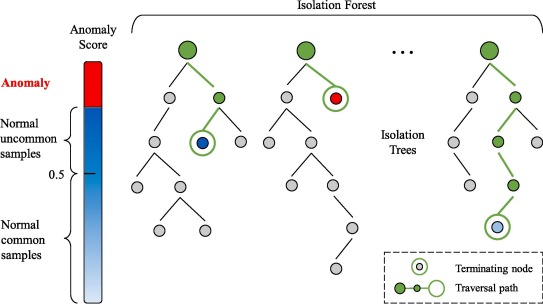
\includegraphics[width=10cm]{fig/Isolation_Forests} % not necessary to give extension - now you can shift between compiling to ps or to pdf without any problems
	
	\caption[Isolation Forest]{Isolation Forests \cite{Chen2020}}
	\label{Figure-Isolation_Forest} 
\end{figure}

The anomaly score is calculated with Eq~\ref{Eq-Isolation_anomaly}
\begin{equation}
s(x,n) = 2^{-E(h(x))/c(n)}
\label{Eq-Isolation_anomaly}
\end{equation}
where $E(h(x))$ is the average value of the distance measured from the tree top for a single data point in all the trees \cite{Hariri2021} and $n$ is the size of a data sample used to train a single tree. For the distance to be normalized, $c(n)$ --- the mean distance from the tree top in an unsuccessful search in a \emph{Binary Search Tree} (BST) --- is used and is calculated as 
\begin{equation}
c(n) = 2H(n-1) - \frac{2(n-1)}{n}.
\label{Eq-normalizing_isolation}
\end{equation}
$H(i)$ in Eq~\ref{Eq-normalizing_isolation} is the harmonic number and is estimated with Euler's constant as 
\begin{equation}
H(i) \approx ln(i) + 0.5772156649.
\label{Eq-H_i}
\end{equation}
Isolation Forests, however have multiple issues, since it splits data in rectangles as seen in Figure~\subref{Figure-ExtendedvsNormal_first}. This is due to the slicing algorithm selecting a feature, $x$ and a cut-off value, $v$. Consequently, the data is either split vertically or horizontally --- if seen as a two dimensional dataset. This split method is unable to categorise complex data structures. These issues however are addressed by \textcite{Hariri2021} and led to the \emph{Extended Isolation Forest} algorithm.

The extended isolation forest algorithm generalises the isolation forest algorithm by applying a slope to each slice. Data points are therefore divided into two groups depending on the "side" of the plane or slice as seen in Figure~\subref{Figure-ExtendedvsNormal_second}.

\begin{figure}[h!tb]
	\centering
	
	\subfloat[][Isolation Forest Slicing example]{
		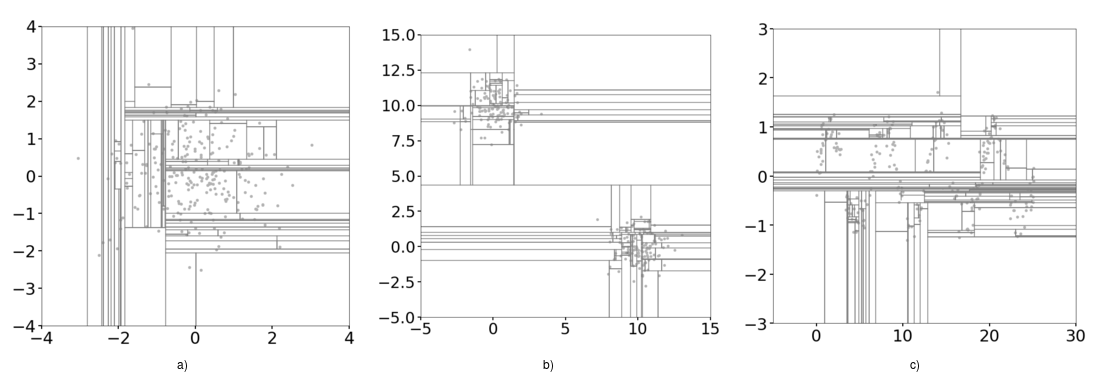
\includegraphics[trim = 0 0 725 0, clip = true, width=7cm]{fig/Isolation_forest_slicing}
		\label{Figure-ExtendedvsNormal_first}
	}
	\quad
	\subfloat[][Extended Isolation Forest Slicing example]{
		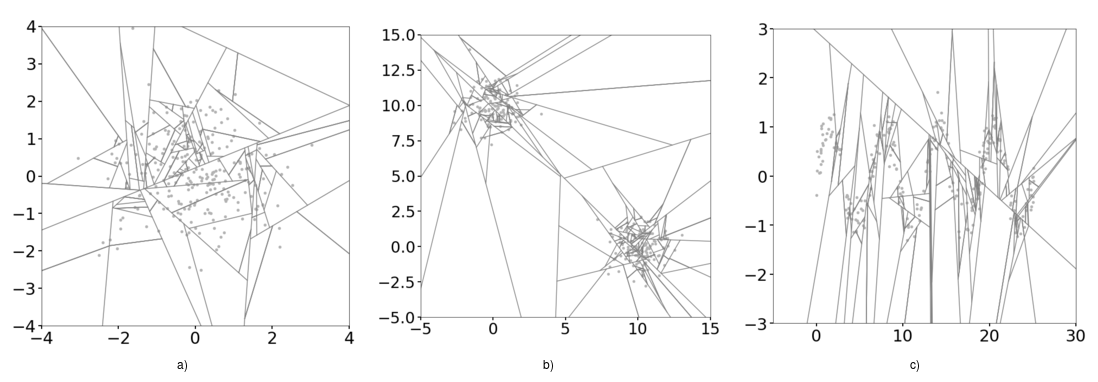
\includegraphics[trim = 0 0 725 0, clip=true,width=7cm]{fig/Extended_Isolation_forest_slicing}
		\label{Figure-ExtendedvsNormal_second}
	}
	\caption[Slicing of Isolation Forest]{The slicing of Isolation Forest vs Extended Isolation Forest}
	\label{Figure-ExtendedvsNormal}
\end{figure}

It is evident that applying an angle of $0\degree$ to all the slices the general algorithm of the extended isolation forest produces the standard isolation forest algorithm where planes or slices are perpendicular to the axis of the randomly selected feature, $x$.

\subsection{Local Outlier Factor}
Most algorithms for anomaly detection are based on a metric which accounts for the entire dataset~\cite{breunig2000lof}. However, many anomalies are identifiable in relation to the local neighbourhood of data points and not the overall dataset. Therefore, \textcite{breunig2000lof} developed the local outlier factor \(LOF\) algorithm that provides a measure of a data point's "outlierness". This implies that a data point is not classified as an anomaly or not, but a local outlier factor is calculated to determine how much a data point is distantiated from it's $k$-nearest neighbours. This is clearly demonstrated in Figure~\ref{Figure-LOF_measure} where the data points which are clustered together have smaller LOF's than data points which are removed from the highly dense areas.

\begin{figure}[h!tb]
	\centering
	
	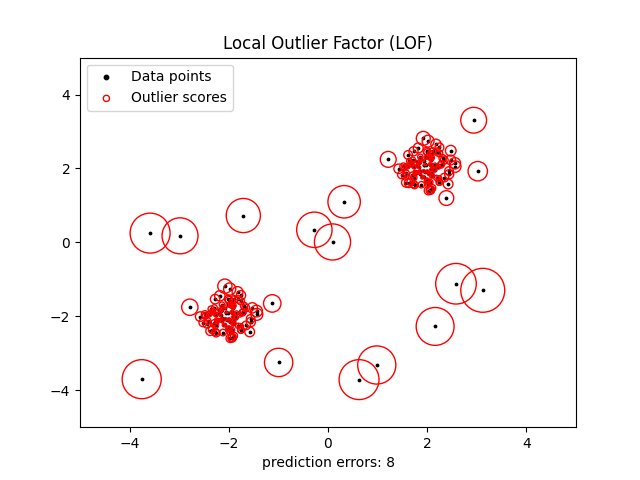
\includegraphics[width=10cm]{fig/LOF_measure} % not necessary to give extension - now you can shift between compiling to ps or to pdf without any problems
	
	\caption[Local outlier measure]{LOF measure}
	\label{Figure-LOF_measure} 
\end{figure}

To calculate the LOF, the $k$-distance must be calculated and also the local reachability density \(lrd\). The $k$-distance, is the $k^{th}$ ranked $distance(o,p_i)$. Where $distance(o,p_i)$ is the distance between data point $o$ and any data point $p_i$, with $i \in N$, where $N$ is the number of data points within the dataset with a minimum value of $MinPts$. To reduce fluctuations in the $distance(o,p_i)$ the distance between $o$ and $p_i$ is replaced with 
\begin{equation}
max \{distance(o,p_i), k\text{-distance}\} 
\end{equation}
and will henceforth be referred to as the reachability distance~\cite{breunig2000lof}. The $lrd$ of a data point, $p$, is calculated as 
\begin{equation}
lrd_{MinPts}(p) = 1/\left(\frac{\sum\limits_{o \in N_{MinPts}(p)}^{} reach\-dist_{MinPts}(p,o)}{|N_{MinPts}(p)|}\right)
\label{Eq-lrd}
\end{equation}
and denotes "the inverse of the average reachability distance based on the $MinPts$-nearest neighbours of the $p$" --- \textcite{breunig2000lof}. Eq~\ref{Eq-lrd} enables the calculation for the $LOF$ of point $p$ as shown in Eq~\ref{Eq-LOF}
\begin{equation}
LOF_{MinPts}(p) = \frac{\sum\limits_{o \in N_{MinPts}(p)}^{}\frac{lrd_{MinPts}(o)}{lrd_{MinPts}(p)}}{|N_{MinPts}(p)|}
\label{Eq-LOF}
\end{equation}
The rule of thumb for detecting an outlier is that when the LOF is larger than 1, then the point is considered an outlier with respect to its neighbourhood. This however is not fixed and the threshold can be changed depending on the application.
This method is aimed at producing a measure of the "outlierness" of a data point within a local neighbourhood and not for all the data points. This method will thus be implemented for the satellite anomaly detection, since it will detect anomalies within the two neighbourhoods produced by the eclipse during orbit. This method will also be able to detect measurements of earth sensors, sun sensors and magnetometers that drastically change from the previous orbital data. For example in Fig~\ref{Figure-Satellite_orbit} it is evident that the LOF will be comparatively larger for the red data points, which are anomalies, to the blue data points that are the normal orbit of the satellite.

\begin{figure}[h!tb]
\centering
\begin{tikzpicture}
\begin{axis}[title = Earth Sensor During Multiple Orbits]
\addplot3 table [x =Earth x, y = Earth y, z=Earth z, col sep=comma, only marks, scatter, blue, fill opacity=0.1, draw opacity = 0]{Data/3D_orbit.csv};
\addplot3 table [x =Earth_anomaly x, y = Earth_anomaly y, z=Earth_anomaly z, col sep=comma, only marks, scatter, red, fill opacity=0.1, draw opacity = 0]{Data/3D_orbit.csv};
\end{axis}
\label{Figure-Satellite_orbit}
\end{tikzpicture}
\end{figure}

\subsection{Kernel Adaptive Density-based}
Kernel adaptive density-based: Is an algorithm that uses the density factor of a data point relative to other data points to determine whether the data point is an outlier or not.

\subsection{Loda}
Loda: Is a fast and efficient anomaly detection algorithm that used histograms to evaluate data points to determine whether a data point is an outlier. Loda is an on-line method and not a batch method.

\subsection{Robust-kernel Density Estimation}
Robust-kernel density estimation

\section{Reinforcement Learning}
Active Anomaly detection with meta-policy (Meta-AAD) is a deep reinforcement learning approcah that is based on the actor-critic model. The agent must query data points within the given dataset (where the queried point is the data top 1 data point). The query is given to a human 


\section{Summary}


	\chapter{Simulation}
% put these two lines after every \chapter{} command
\vspace{-2em}
\minitoc
To implement and research various FDIR systems on satellites an simulation of satellite dynamics and kinematics is developed. The focus of this thesis is on small satellites and more specifically cubesats. For the simulation of the ADCS of the satellite \cite{auret2012design, JansevanVuuren2015, Jordaan2016} were referenced during the development of the satellite simulation. The simulation was developed in Python to simulate the dynamics and kinematics during a satellite orbit. The faults for the subsystems are also developed within the simulation and will be discussed within this chapter.

\section{ADCS}

\subsection{Coordinate Frames}


The main operational goal of the ADCS on this specific satellite mission is to control the payload to point towards the centre of the earth. 

\subsection{Euler Angles and Quaternions}

\subsection{Satellite Kinematics and Dynamics}

\subsection{Rungka-kutta}

\section{Environment}
\subsection{Earth Orbit}
Earth orbit according to sgp4 and also the placement of the earth sensor.

Show plot of 3D earth orbit...

\subsection{Sun}
The calculations for the sun position and also the placement of the coarse and fine sun sensor.

\subsection{Geomagnetic field}

\begin{equation}
V(r_s,\theta, \lambda) = R_E \sum_{n=1}^{k}\left(\frac{R_E}{r_s}^{n+1}\right)\sum_{m=0}^{n}\left(g_n^mcos(m\lambda) + h_n^msin(m\lambda)\right)P_n^m(\theta)
\end{equation}

Show graph of geomagnetic plot...

\section{Sensor models}
\subsection{Position of Sensors and Field of View}

\begin{figure}
\centering
\begin{tikzpicture}[tdplot_main_coords]
		% Start of cone
		\coordinate (O) at (0,0,0.5);
		
		%% make sure to draw everything from back to front
		%\coneback[surface]{-1.5}{2.5}{-15}
		%\coneback[surface]{-3}{2}{-10}
		\draw (0,0,-5) -- (O);
		%\conefront[surface]{-3}{2}{-10}
		%\conefront[surface]{-1.5}{2.5}{-15}
		%\filldraw[surface] circle (3);
		\draw[->] (-6,0,0) -- (6,0,0) node[right] {$x$};
		\draw[->] (0,-6,0) -- (0,6,0) node[right] {$y$};
		
		%\coneback[surface]{3}{2}{10}
		\draw[->] (O) -- (0,0,5) node[above] {$z$};

	%%% Edit the following coordinate to change the shape of your
%%% cuboid

%% Vanishing points for perspective handling
\coordinate (P1) at (-7cm,1.5cm); % left vanishing point (To pick)
\coordinate (P2) at (8cm,1.5cm); % right vanishing point (To pick)

%% (A1) and (A2) defines the 2 central points of the cuboid
\coordinate (A1) at (0em,0cm); % central top point (To pick)
\coordinate (A2) at (0em,-2cm); % central bottom point (To pick)

%% (A3) to (A8) are computed given a unique parameter (or 2) .8
% You can vary .8 from 0 to 1 to change perspective on left side
\coordinate (A3) at ($(P1)!.8!(A2)$); % To pick for perspective 
\coordinate (A4) at ($(P1)!.8!(A1)$);

% You can vary .8 from 0 to 1 to change perspective on right side
\coordinate (A7) at ($(P2)!.7!(A2)$);
\coordinate (A8) at ($(P2)!.7!(A1)$);

%% Automatically compute the last 2 points with intersections
\coordinate (A5) at
(intersection cs: first line={(A8) -- (P1)},
second line={(A4) -- (P2)});
\coordinate (A6) at
(intersection cs: first line={(A7) -- (P1)}, 
second line={(A3) -- (P2)});

%%% Depending of what you want to display, you can comment/edit
%%% the following lines

%% Possibly draw back faces

\fill[gray!90] (A2) -- (A3) -- (A6) -- (A7) -- cycle; % face 6
\node at (barycentric cs:A2=1,A3=1,A6=1,A7=1) {\tiny f6};

\fill[gray!50] (A3) -- (A4) -- (A5) -- (A6) -- cycle; % face 3
\node at (barycentric cs:A3=1,A4=1,A5=1,A6=1) {\tiny f3};

\fill[gray!30] (A5) -- (A6) -- (A7) -- (A8) -- cycle; % face 4
\node at (barycentric cs:A5=1,A6=1,A7=1,A8=1) {\tiny f4};

\draw[thick,dashed] (A5) -- (A6);
\draw[thick,dashed] (A3) -- (A6);
\draw[thick,dashed] (A7) -- (A6);

%% Possibly draw front faces

% \fill[orange] (A1) -- (A8) -- (A7) -- (A2) -- cycle; % face 1
% \node at (barycentric cs:A1=1,A8=1,A7=1,A2=1) {\tiny f1};
\fill[gray!50,opacity=0.2] (A1) -- (A2) -- (A3) -- (A4) -- cycle; % f2
\node at (barycentric cs:A1=1,A2=1,A3=1,A4=1) {\tiny f2};
\fill[gray!90,opacity=0.2] (A1) -- (A4) -- (A5) -- (A8) -- cycle; % f5
\node at (barycentric cs:A1=1,A4=1,A5=1,A8=1) {\tiny f5};

%% Possibly draw front lines
\draw[thick] (A1) -- (A2);
\draw[thick] (A3) -- (A4);
\draw[thick] (A7) -- (A8);
\draw[thick] (A1) -- (A4);
\draw[thick] (A1) -- (A8);
\draw[thick] (A2) -- (A3);
\draw[thick] (A2) -- (A7);
\draw[thick] (A4) -- (A5);
\draw[thick] (A8) -- (A5);

% Possibly draw points
% (it can help you understand the cuboid structure)
\foreach \i in {1,2,...,8}
{
	\draw[fill=black] (A\i) circle (0.15em)
	node[above right] {\tiny \i};
}
		\coneback[surface]{1.5}{2.5}{15}
		\conefront[surface]{1.5}{2.5}{15}
\end{tikzpicture}
\end{figure}

\tdplotsetmaincoords{70}{120}
\begin{figure}
\centering
\begin{tikzpicture}[tdplot_main_coords]
\def\BigSide{5}
\def\SmallSide{1.5}
\pgfmathsetmacro{\CalcSide}{\BigSide-\SmallSide}

% The vertex at V
\tdplotsetcoord{P}{sqrt(3)*\BigSide}{55}{45}

\coordinate (sxl) at (\BigSide,\CalcSide,\BigSide);
\coordinate (syl) at (\CalcSide,\CalcSide,\BigSide);
\coordinate (szl) at (\CalcSide,\BigSide,\BigSide);

\draw[dashed] 
(0,0,0) -- (Px)
(0,0,0) -- (Py)
(0,0,0) -- (Pz);
\draw[->] 
(Px) -- ++ (1,0,0) node[anchor=north east]{$x$};
\draw[->]
(Py) -- ++(0,1,0) node[anchor=north west]{$y$};
\draw[->] 
(Pz) -- ++(0,0,1) node[anchor=south]{$z$};

\draw[thick]
(Pxz) -- (P) -- (Pxy) -- (Px) -- (Pxz) -- (Pz) -- (Pyz) -- (P); 
\draw[thick]
(Pyz) -- (Py) -- (Pxy);


\end{tikzpicture}
\end{figure}


\subsection{Disturbance models}
\subsubsection{Gravity Gradient}

\subsubsection{Aerodynamic Disturbance}

\subsubsection{Wheel Imbalance}

\section{Attitude Determination}
IN this chapter discuss the Kalman filter.

\section{Attitude Control}
Magnetic control during detumbling
Reaction wheel control during normal operation

\section{Typical Faults}
For the simulation of the satellite and the induced faults to train and test various anomaly detection methodologies a database of typical faults is required. \textcite{tafazoli2009study} made a study of the percentage of failure per subsystem. 

\subsubsection{Faults}
The occurrence of a fault depends on the reliability of that equipment. \textcite{Guo2014} studied the reliability of small satellites and calculated the parameters for the Weibull distribution based on real data. A set of typical faults for the ADCS is shown in Table~\ref{ADCS fault table}. 

\newpage
\begin{sidewaystable}[]
	\label{ADCS faults}
	\begin{tabular}{|l|c|l|l|l|l|}
		\hline
		\multicolumn{6}{|c|}{\textbf{Internal Faults}} \\ \hline
		\textbf{Fault classes} &
		\multicolumn{1}{l|}{\textbf{\begin{tabular}[c]{@{}l@{}}Failure rate \\ per hour\end{tabular}}} &
		\textbf{Fault causes} &
		\textbf{References} &
		\textbf{Possible effect} &
		\textbf{Possible permutations} \\ \hline
		\multirow{4}{*}{Reaction wheels} &
		\multicolumn{1}{l|}{\multirow{4}{*}{2.5E-7 \cite{Spilhaus1987}}} &
		\begin{tabular}[c]{@{}l@{}}Reaction wheel electronics \\ fail\end{tabular} &
		\cite{allen2012satellite} \cite{Jacklin2019} &
		\begin{tabular}[c]{@{}l@{}}Does not respond \\ to control inputs\end{tabular} &
		\begin{tabular}[c]{@{}l@{}}Momentum remains the same \\ or decreases slightly due to \\ friction\end{tabular} \\ \cline{3-6} 
		&
		\multicolumn{1}{l|}{} &
		Overheated reaction wheel &
		\cite{Wintoft} &
		Decrease in speed &
		1\% of initial speed per second \\ \cline{3-6} 
		&
		\multicolumn{1}{l|}{} &
		\begin{tabular}[c]{@{}l@{}}Catastrophic failure (cause \\ unknown)\end{tabular} &
		\cite{Choi2011} &
		Stops rotating &
		0 \\ \cline{3-6} 
		&
		\multicolumn{1}{l|}{} &
		\begin{tabular}[c]{@{}l@{}}Increase in rotation speed \\ (Unknown cause)\end{tabular} &
		\begin{tabular}[c]{@{}l@{}}Gerhard Janse \\ van Vuuren\end{tabular} &
		\begin{tabular}[c]{@{}l@{}}Wheel speed \\ increases\end{tabular} &
		\begin{tabular}[c]{@{}l@{}}Between 90-100\% of maximum \\ wheel speed\end{tabular} \\ \hline
		Magnetorquers &
		\multicolumn{1}{l|}{8.15E-9 \cite{Spilhaus1987}} &
		Polarities are inverted &
		\cite{Crowell2011} &
		Incorrect rotation &
		\\ \hline
		\multirow{2}{*}{Magnetometers} &
		\multicolumn{1}{l|}{\multirow{2}{*}{8.15E-9 \cite{Spilhaus1987}}} &
		Unknown &
		\begin{tabular}[c]{@{}l@{}}Gerhard Janse \\ van Vuuren\end{tabular} &
		Stops reacting &
		\begin{tabular}[c]{@{}l@{}}Provides no feedback or the \\ output remains constant\end{tabular} \\ \cline{3-6} 
		&
		\multicolumn{1}{l|}{} &
		\begin{tabular}[c]{@{}l@{}}Magnetometers and magne-\\ torquers interfered with \\ each other\end{tabular} &
		\cite{Jacklin2019} &
		\begin{tabular}[c]{@{}l@{}}Noise on magneto-\\ meters and noise \\ on control of mag-\\ netorquers\end{tabular} &
		\begin{tabular}[c]{@{}l@{}}Between x3 and x5 times the \\ normal noise magnitude \\ Guassian distribution\end{tabular} \\ \hline
		Earth Sensor &
		- &
		Unknown &
		\cite{Robertson2019} &
		\begin{tabular}[c]{@{}l@{}}Noisy Earth Sensor \\ effected pointing \\ accuracy\end{tabular} &
		\begin{tabular}[c]{@{}l@{}}Between x5 and x10 times the \\ normal sensor noise based on \\ Guassian distribution\end{tabular} \\ \hline
		\multirow{2}{*}{Sun sensor} &
		\multirow{2}{*}{-} &
		\begin{tabular}[c]{@{}l@{}}Cross-wired during instal-\\ lation\end{tabular} &
		\cite{Crowell2011} &
		\begin{tabular}[c]{@{}l@{}}Erroneous \\ measurements\end{tabular} &
		Uniform random values \\ \cline{3-6} 
		&
		&
		Unknown &
		\cite{Jacklin2019} &
		Sun sensor fails &
		output is 0 \\ \hline
		Star tracker &
		- &
		\begin{tabular}[c]{@{}l@{}}Shutter on star tracker is \\ closed\end{tabular} &
		\cite{Crowell2011} &
		Star tracker fails &
		output is 0 \\ \hline
		Overall control &
		- &
		\begin{tabular}[c]{@{}l@{}}Incorrect control law or \\ variation \\ thereof\end{tabular} &
		\begin{tabular}[c]{@{}l@{}}Gerhard Janse \\ van Vuuren\end{tabular} &
		\begin{tabular}[c]{@{}l@{}}Angular velocity \\ suddenly increases \\ or decreases or \\ oscillation results\end{tabular} &
		\begin{tabular}[c]{@{}l@{}}Increase to 75 - 100\% \\ Decrease to 0 - 25\%\\ Oscillates\end{tabular} \\ \hline
		\multirow{3}{*}{\begin{tabular}[c]{@{}l@{}}Common data \\ transmission errors\end{tabular}} &
		\multirow{3}{*}{-} &
		Sign flip &
		\cite{Crowell2011} &
		Processor-based &
		\begin{tabular}[c]{@{}l@{}}Processor outputs and/or \\ inputs experience a sign flip\end{tabular} \\ \cline{3-6} 
		&
		&
		Bit flip &
		N/A &
		&
		\begin{tabular}[c]{@{}l@{}}Processor outputs and/or \\ inputs experience a bit flip flip\end{tabular} \\ \cline{3-6} 
		&
		&
		Insertion of zeros &
		\cite{Jacklin2019} &
		&
		\begin{tabular}[c]{@{}l@{}}Processor outputs and/or inputs \\ experience an insertion of a zero\end{tabular} \\ \hline
		\begin{tabular}[c]{@{}l@{}}Possible sensors \\ errors\end{tabular} &
		- &
		Unknown &
		N/A &
		High sensor noise &
		\begin{tabular}[c]{@{}l@{}}Between x5 and x10 times the \\ normal sensor noise based on \\ Guassian distribution\end{tabular} \\ \hline
	\end{tabular}
	\label{ADCS fault table}
\end{sidewaystable}

\newpage
	\chapter{Implementation of Methods on Actual Satellite}
% put these two lines after every \chapter{} command
\vspace{-2em}
\minitoc

\section{Isolation Forests}
A trained network will be developed from simulation data or the data generated during the first few orbits of a satellite. Afterwards the anomaly score will be calculated for a data point and based on a given threshold, the data point will be flagged as an anomaly or not.
	%%%%%%%%%%%%%%%%%%%%%%%%%%%%%%%%%%%%%%%%%%%%%%%%
%
% start writing
%
%%%%%%%%%%%%%%%%%%%%%%%%%%%%%%%%%%%%%%%%%%%%%%%%


\chapter{Conclusion}
% put these two lines after every \chapter{} command
\vspace{-2em}
\minitoc

%\startarabicpagenumbering % must be just after the first \chapter{} command


\blindtext

\section{Project/thesis/dissertation summary}

\blindtext

\blindtext

\section{Appraisal of project/thesis/dissertation contributions}

\blindtext

\section{Suggestions for future work}

\blindtext

\section{What the student has learnt during this project}		%ONly for skripsie students

\blindtext
	
	%=================================================
	% bibliography
	%=================================================
	%\cite{*} % cites all items in your .bib file for the purpose of testing biblatex - REMOVE!
	\printbibliography[heading=bibintoc]
	
	
	%=================================================
	% Appendices
	%=================================================
	\appendix
	\chapter{Project Timeline}

The expected timeline is given in Figure \ref{Ganttchart} in Gantt-chart form.


\begin{figure}[htb]
\centering
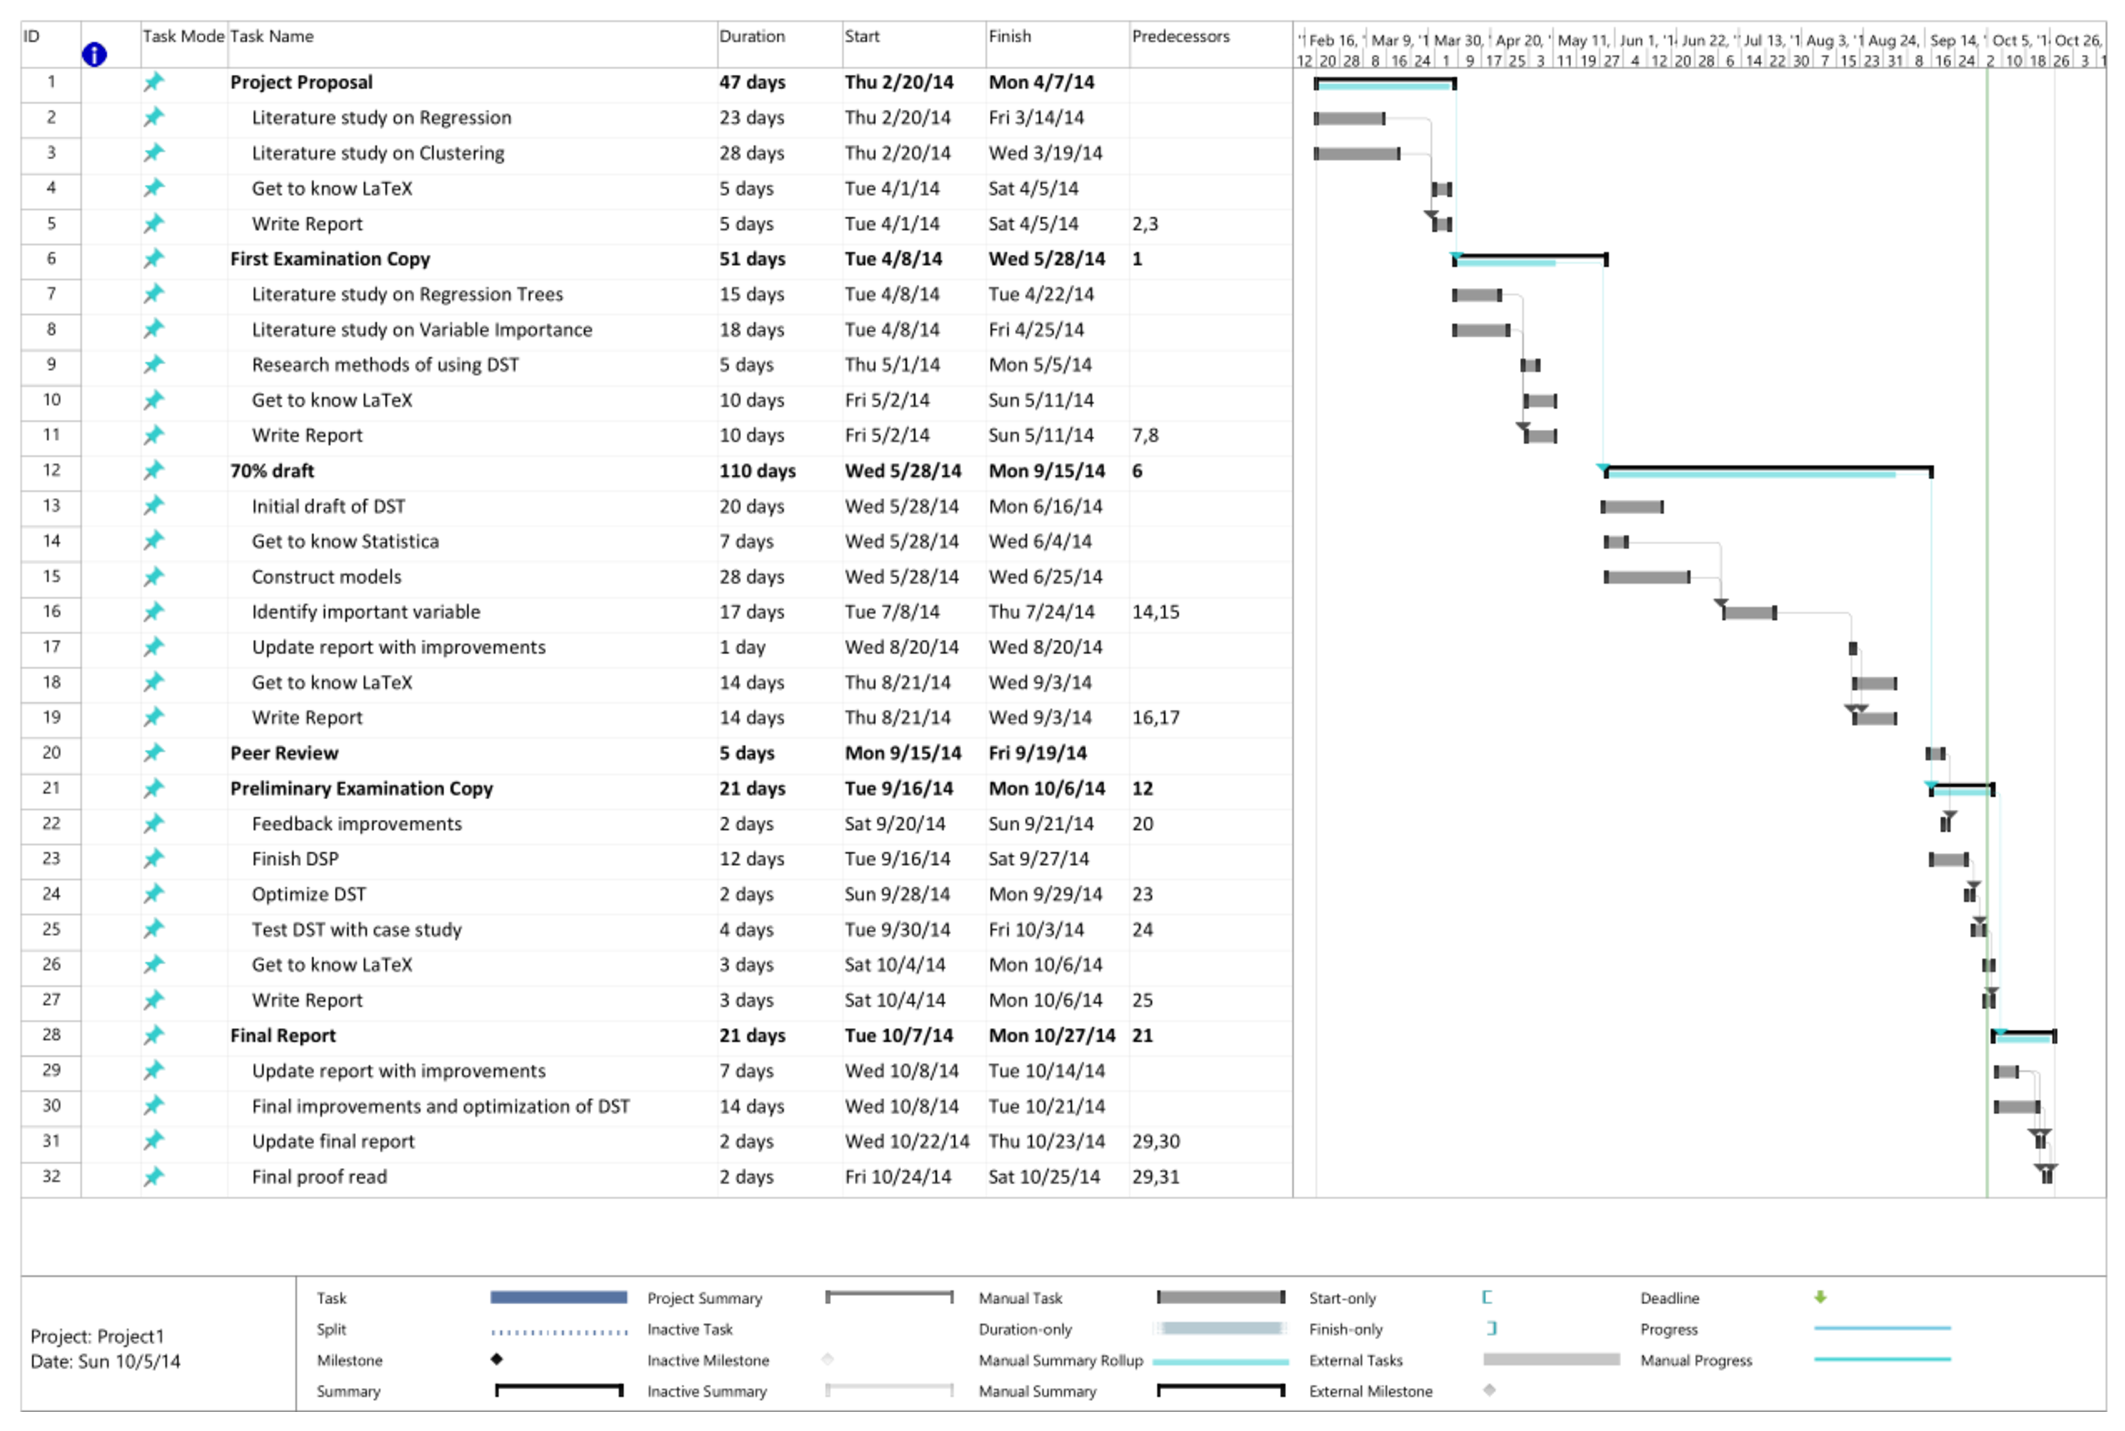
\includegraphics[angle=90,scale=0.6,trim=0 0 0 0, clip]{fig/Timeline}
%\leftskip-1.5cm
\caption{Expected timeline in Gannt-chart form.}
\label{Ganttchart}
\end{figure}
	\chapter{Data}

% EXAMPLE
%=========
%
% example using multicolumn, multirow and the sideways environment
Data related to the Case Study in Chapter 5 are presented in Table \ref{ex2}.
\begin{table}[h!tb]

\centering

\begin{tabular}{cc|rrrrrr}\hline

\headcol &&\multicolumn{6}{c}{this goes across 6 columns}\\

 \headcol && col a & col b & col c & col d & col e & col f \\ \hline \hline

\multirow{6}{*}{
%
\begin{sideways}
this is sideways,
\end{sideways}
%
\begin{sideways}
and goes across
\end{sideways}
%
\begin{sideways}
six rows
\end{sideways}
%
}


& row 1 \\
& row 2 & \cellcolrow & \cellcolrow & \cellcolrow & \cellcolrow & \cellcolrow & \cellcolrow \\
& row 3 \\ 
& row 4 & \cellcolrow & \cellcolrow & \cellcolrow & \cellcolrow & \cellcolrow & \cellcolrow \\
& row 5 \\
& row 6 & \cellcolrow & \cellcolrow & \cellcolrow & \cellcolrow & \cellcolrow & \cellcolrow \\ \hline

\end{tabular}

\caption[Do not end short caption with full-stop]{Type full caption here.}
\label{ex2}

\end{table}

	
	
\end{document}
